
\begin{frame}
    \frametitle{Future of Meteor Radar}
    \begin{columns}
        \begin{column}{0.65\textwidth}
            \textit{Eventual goals include:} \\ ~ \\ 
                        \alert{Wide-scale MLT coverage through continental networks}
            \begin{itemize}
                \footnotesize
                \item[$\blacktriangleright$] Atmosphere evolves over huge spans of space and time 
                \item[$\blacktriangleright$] Understanding large-scale dynamics require large-scale observations
                \item[$\blacktriangleright$] Achievable through moderate investments in infrastructure
            \end{itemize}            
        \end{column}
        \begin{column}{0.35\textwidth}
            \begin{tikzpicture}[anchor=(current bounding box.center)]
                \node[anchor=center, inner sep=0] (img) at (0,0) {
                    {{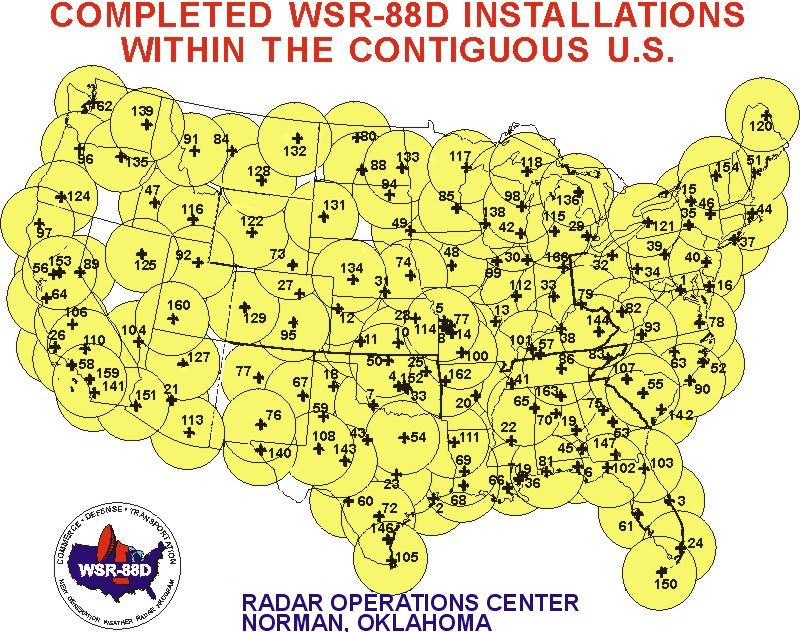
\includegraphics[width=\linewidth]{img/NEXRAD_NETWORK.jpg}}}
                };
                \node[anchor=north, inner sep=2pt] at ([yshift=-0.3cm]img.north) { 
                    {{{\fontsize{3}{3.4}\selectfont\raggedleft \textcolor{black}{\textit{Credit:} \cite{nasaglobalhydrometeorologyresourcecenterdaac_NEXRADIMPACTSDatasets_2023}}}}}
                };
            \end{tikzpicture}
            \footnotesize
            \textit{Continental-scale tropospheric observations enable reliable weather forecasting}
        \end{column}
    \end{columns}
\end{frame}